%\documentclass[12pt,man,fignum,floatmark]{apa}
\documentclass[12pt]{article}
\usepackage{url,epsfig,apacite,lineno,booktabs,rotating,setspace,amsmath,bm}
\usepackage{tabu}
\usepackage{caption}
\usepackage{fancyvrb,framed}
\usepackage[normalem]{ulem}
\usepackage{amsmath}
\usepackage{amsfonts}
\usepackage{amssymb}

\interfootnotelinepenalty=10000
\widowpenalty=10000
\clubpenalty = 10000


\title{Classification models part}
\author{Yuxiao Wang}


\begin{document}

%\setcounter{page}{0}
\pagestyle{plain}

\maketitle
\section{Classification of response vs non-response}
In this section, we consider the problem of predicting the response (yes or no) based on the characteristics of the patients. In this work, we mainly focus on the t\_baseline features and the t\_concentration features, both of which are measures of the brain image in different regions. 

\section{Classification models}
There is no single model that can work well for all datasets. In this work, we evaluated different types of classification algorithms in order to find the ones that are most suitable for this problem. Specifically, we consider the following classification models. 
\begin{itemize}  \setlength\itemsep{0em}

\item k nearest neighbors (kNN): the prediction is based on the majority vote by labels of the neighboring training data.
\item support vector machine (SVM): a discriminative classifier defined by a  separating hyperplane, where the margin of the training data is maximized. Multiple kernels can be used to incorporate features of more complex structures. Popular kernels include linear kernel,  polynomial kernel and RBF(Gaussian) kernel.
\item Gaussian process: a classifier based on Gaussian process. 
\item Decision tree: an algorithm that recursively breaks down the training set into smaller pieces according to one feature at each time, and thus constructing a tree-structured model, where the prediction is computed via the leaf nodes.
\item Random forest: ensemble of decision trees that are constructed using a subset of the features and training data. It usually has better performance comparing to decision tree as it reduces the possibility of model overfitting.
\item Multilayer perceptron: a feedforward artificial neural network model that maps the input data to output through multiple hidden layers.
\item AdaBoost: uses a sequence of weak learners that are tweaked in favor of the error made by the previous learners.
\item Naive Bayes: a simple Bayesian classifiers where the features are assumed to be independent conditional on the classification labels.
\item Quadratic discriminant analysis: the algorithm is similar to linear discriminant analysis (LDA) but there are no assumptions on the covariance matrices.
\end{itemize}

\subsection{Model evaluation}
The dataset is randomly split into training and testing data, where the testing data contains about 20\% of the data while the training data consists of the rest 80\%. The model training is purely based on the training data and the evaluation is performed on the testing data. The performance of the model is evaluated by the accuracy, which is the proportion of the testing data that the model gives the correct prediction. 

\subsection{Result}
Table \ref{table:classification_accuracy} displays the classification accuracy for the classification algorithms.  All of the classification accuracy is around 50\%, which means all the models are no better than random guessing. Considering that the labels are not balanced, the models actually perform worse than just predicting $1$ for all test samples. Figure \ref{fig:decision_boundary} shows the decision boundary for the models,  plotted on a 2-D space spanned by the first two principal components. The projection onto the space spanned by the first two principal components accounts for  70\% of the total variation. It is observable that the two classes are overlapping and are not linearly separable. 

The results show that non of the single model has a reasonably well performance.  Though disappointing, it does not necessarily mean that the models are useless for this problem, as the results are obtained for single model that are trained on raw features (no transformations at all). Better feature engineering, model stack and ensembling could boost the performance, when there are enough training samples. Moreover, the output of the models can be informative, for example, random forest model can also rank the importance of the input features.




\begin{table}[h]


\begin{tabular}{lrrr}
\toprule
                      model\_name &  only t\_baseline &  only t\_concentration &      both \\
\midrule
               Nearest Neighbors &         0.492147 &              0.518325 &  0.492147 \\
                      Linear SVM &         0.481675 &              0.528796 &  0.481675 \\
                         RBF SVM &         0.523560 &              0.523560 &  0.523560 \\
                Gaussian Process &         0.481675 &              0.518325 &  0.518325 \\
                   Decision Tree &         0.554974 &              0.460733 &  0.513089 \\
                   Random Forest &         0.513089 &              0.544503 &  0.539267 \\
           Multilayer Perceptron &         0.486911 &              0.502618 &  0.481675 \\
                        AdaBoost &         0.465969 &              0.476440 &  0.513089 \\
                     Naive Bayes &         0.492147 &              0.465969 &  0.455497 \\
 Quadratic Discriminant Analysis &         0.539267 &              0.560209 &  0.507853 \\
\bottomrule
\end{tabular}
\caption{Evaluation of the classification accuracy of different models.}
\label{table:classification_accuracy}
\end{table}

\begin{figure}
  \centering
    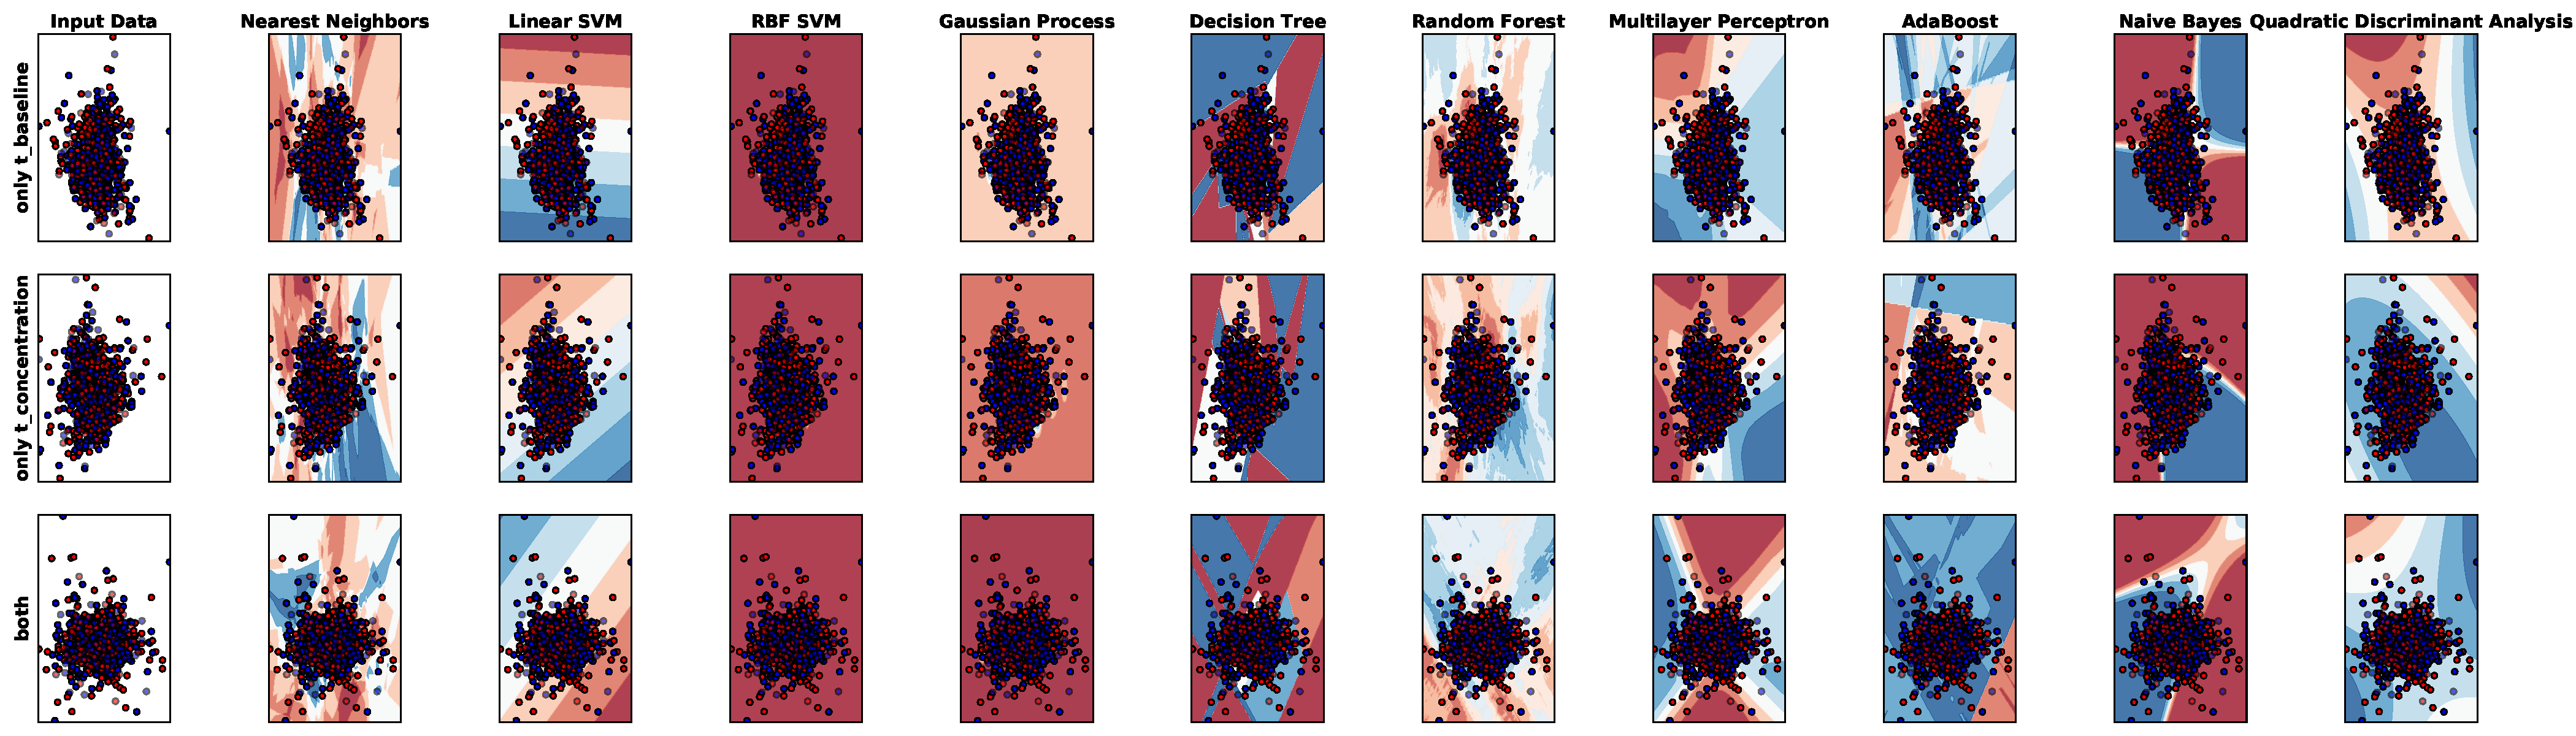
\includegraphics[width=1.2\textwidth]{./figure/classification_result.pdf}
      \caption{Decision boundary for the classifiers.}
      \label{fig:decision_boundary}
\end{figure}



\end{document}











